\subsection{Event Match Rate}
%\textbf{Text Event Match.} 
To evaluate the alignment between predicted clinical events and reference annotations, we used a recursive best-match strategy adopted from our previous work \citep{wang2025large}. This method pairs events by minimizing string-based distances while avoiding many-to-one mappings. For each reference event, the closest predicted event is selected based on the minimal distance, with text order, \emph{i.e.}, the order of the events in the annotation files, to break distance ties. Once matched, both events are removed from further consideration, and the process continues recursively with the remaining pairs. \textcolor{red}{George: how does this greedy approach do compared to the classical 1955 Hungarian algorithm (we would use this to match predicted clinical events to reference ones, where if there is a mismatch in the numbers, e.g., more reference ones than predicted ones, you just introduce ``empty'' predicted ones that have 0 cost)? Also, is there some way to use an evaluation metric like optimal transport distance?}

We tested several distance metrics, including Levenshtein distance, cosine similarity of \texttt{BERT} (\texttt{bert-base-uncased}) embeddings, and cosine similarity based on sentence embeddings from \texttt{PubMedBERT} (\texttt{S-PubMedBert-MS-MARCO}). Previous validation showed that \texttt{PubMedBERT-based} cosine similarity with a threshold of 0.1 was the most reliable, and we used this metric for our evaluation. The detailed pseudo code of the recursive best match algorithm is provided in Algorithm~\ref{alg:recursive_match}. \textcolor{red}{George: Where does the threshold show up in Algorithm~1? How is the final event match rate defined (is it just the fraction of reference events that are matched, i.e., recall? precision? F1? something else?)?}
% We provide pseudocode for the best match procedure between two lists of strings (Algorithm \ref{alg:recursive_match}).  For each list, we use the text order, \emph{i.e.}, the order of the events in the annotation files, to break embedding distance ties.  We use the cosine similarity for the distance calculation using sentence transformer embeddings from \texttt{S-PubMedBert-MS-MARCO}.

\begin{algorithm}[ht]
\caption{Recursive Best Match}
\scriptsize
\label{alg:recursive_match}
\begin{algorithmic}[1]
\Require Two lists: \texttt{ref} (manually annotated reference events) and \texttt{pred} (predicted events)
\Ensure List of best-matching event pairs
\Function{MatchEvents}{\texttt{ref}, \texttt{pred}}
    \If{\texttt{ref} is empty \textbf{or} \texttt{pred} is empty}
        \State \Return \texttt{[]}
    \EndIf
    \State $\texttt{min\_distance} \gets \infty$
    \State $\texttt{best\_pair} \gets \texttt{None}$
    \ForAll{$r \in \texttt{ref}$}
        \ForAll{$p \in \texttt{pred}$}
            \State $d \gets \texttt{ComputeDistance}(r, p)$
            \If{$d < \texttt{min\_distance}$}
                \State $\texttt{min\_distance} \gets d$
                \State $\texttt{best\_pair} \gets (r, p)$
            \ElsIf{$d = \texttt{min\_distance}$}
                \State $(r^*, p^*) \gets \texttt{best\_pair}$
                \State Get indices (within the annotation files) of $r$, $p$, and also of $r^*, p^*$
                \If{index of $r <$ index of $r^*$}
                    \State $\texttt{best\_pair} \gets (r, p)$
                \ElsIf{index of $r = $ index of $r^*$ \textbf{and} index of $p <$ index of $p^*$}
                    \State $\texttt{best\_pair} \gets (r, p)$
                \EndIf
            \EndIf
        \EndFor
    \EndFor
    \State $(r^*,p^*) \gets \texttt{best\_pair}$
    \State Remove $r^*$ from \texttt{ref}
    \State Remove $p^*$ from \texttt{pred}
    \State $\texttt{result} \gets \texttt{[best\_pair]} + \texttt{MatchEvents}(\texttt{ref}, \texttt{pred})$
    \State \Return $\texttt{result}$
\EndFunction
\end{algorithmic}
\end{algorithm}

\subsection{Temporal Concordance}
%\textbf{Temporal Ordering.} 
To quantify the accuracy of temporal ordering, we used the concordance index (c-index), which measures the probability that a randomly selected pair of predicted events is correctly ordered in time (so c-index values range from 0 to 1). Higher c-index values indicate better alignment with the reference timeline. Formally, suppose that for a specific case report (corresponding to a single patient) that we have a manual annotation for, after doing the matching described in the previous section, we find that there are a total of $k$ events that matched. For event $i\in\{1,2,\dots,k\}$, we denote the (manually annotated) reference time for event $i$ as $t_i^{\text{ref}}$ and the LLM-extracted time as $t_p^{\text{pred}}$. Then the c-index is calculated as
\[
\text{c-index} = \frac{1}{N} \sum_{i,j\in\{1,2,\dots,k\}\text{ s.t.~}i<j} {\mathds{1}\{(t^{\text{ref}}_i - t^\text{ref}_j)(t^{\text{pred}}_i - t^{\text{pred}}_j) > 0\}},
\]
where $\mathds{1}\{\cdot\}$ is the indicator function, and $N$ is the number of ``comparable'' pairs (a pair of events $(i,j)$ with $i<j$ is comparable if $t^{\text{ref}}_i \neq t^{\text{ref}}_j$ and $t^{\text{pred}}_i \neq t^{\text{pred}}_j$).

% \vspace{-10pt}
% \begin{equation}
% \text{c-index} = \frac{1}{N} \sum_{i<j} \mathbf{1}[(t^r_i - t^r_j)(t^p_i - t^p_j) > 0]
% \end{equation}
% \vspace{-10pt}

\subsection{Time Discrepancy}
%\textbf{Time Discrepancy Analysis.} 
We evaluated temporal prediction accuracy by measuring the discrepancies between predicted and reference times. Continuing to use notation from the previous section, note that for a specific matched event, the absolute difference in predicted and reference times is $|t_i^{\text{pred}} - t_i^{\text{ref}}|$. If we denote any such absolute time difference as $\Delta t$ (in hours), then we specifically measure the \emph{log-time discrepancy} defined as $\log(1 + \Delta t)$. To summarize these discrepancies, we introduce the Area Under the Log-Time Cumulative Distribution Function (AULTC), which quantifies how quickly the cumulative distribution of log-time discrepancy values rises---higher AULTC values indicate better temporal alignment. The full definition of AULTC is in Appendix \ref{apd:ltcdf}. We also stratified the analysis by different time granularities (hour, day, week, year) to examine how prediction accuracy varies with time from case presentation. \textcolor{red}{George: In constructing the empirical distribution function, do you use log-time discrepancy values across the entire ``gold set''?}

%%%%%%%%%%%%%%%%%%%%%%%%%%%
%%%%%%%%%%%%%%%%%%%%%%%%%%%
\section{Log-Time Cumulative Distribution Function}
\label{apd:ltcdf}
\textcolor{red}{George: In Appendix A, why is there even text regarding non-convexity? Why is this important for the reviewer/reader to know? When training neural nets in practice, I'm under the impression that the vast majority of loss functions used aren't actually convex (for example, even though MSE loss on its own is convex, once you compose it with the rest of a neural net used, the overall loss is usually no longer convex with respect to the neural network parameters/"weights"). I just find this part to be superfluous and to not convey useful theoretical insight. Perhaps I'm missing something?}

Recall the log-time cumulative distribution function is given as follows:

% \subsection{baal}
% \subsubsection{baal1}
\[
   F(x) = \frac{1}{k} \sum_{i=1}^k \mathds{1}\{x_{(i)} \leq x\},
\]
where $\mathds{1}$ is the indicator function.

We compute the AULTC as the area under $F(x)$ from $x = 0$ to $x = \log(1 + S_{\text{max}})$, normalized by $\log(1 + S_{\text{max}})$:
\begin{align*}
\text{AULTC} &= \frac{1}{\log(1 + S_{\text{max}})} \Bigg[ \sum_{i=1}^k (x_{(i)} - x_{(i-1)}) \frac{i}{k} + (\log(1 + S_{\text{max}}) - x_{(k)}) \times 1 \Bigg]
\end{align*}
where $x_{(0)} = 0$. With this definition, AULTC = 1 indicates that discrepancies are zero (perfect recovery), resulting in maximum area $\log(1 + S_{\text{max}})$, and AULTC = 0 indicates that all discrepancies exceed $S_{\text{max}}$, yielding zero area. 
% The code for the AULTC calculation is given in the function \texttt{ecdf\textunderscore auc2(\dots)} in the Supplementary Materials.


\begin{remark}
The time unit and cutoff $S_\text{max}$ affect the AULTC calculation, so they must be specified when reporting the AULTC.
\end{remark}

Because of the $\log(1 + \cdot)$ transformation (rather than the $\log(\cdot)$ transformation which is undefined for zero time-error discrepancy), the discrepancies are non-linearly shifted in the log scale.  The non-linear shift adjusts the relative widths of the step function (particularly for small discrepancies) changing the area calculation.  The cutoff $S_\text{max}$ affects the normalization factor.  Therefore, these values should be chosen based on practicalities for the application.  In our case, we chose hours at the time unit because the only sub-hour descriptions reported were several Apgar scores at the minute-level.

\begin{remark}
    The average log-time discrepancy is non-convex.
\end{remark}
This can be seen from the observation that the $\log(1+\cdot)$ function is ``spikier'' than the L1 function. More formally, the log-time discrepancy has a higher curvature around zero error compared to the L1 loss. Consider the second derivatives of the loss functions with respect to the discrepancies $s = |t^p - t^r|$.  For L1 loss $L_1(s) = s$, the second derivative $\frac{d^2 L_1}{ds^2} = 0$ for $s > 0$.
For the log-time loss, $L_{log}(s) = \log(1 + s)$, the second derivative is $\frac{d^2 L_{log}}{ds^2} = -\frac{1}{(1 + s)^2}$. At $s = 0$, the second derivative is $-1$, while the second derivative of the L1 loss is $0$.

To provide a simple counterexample, define the average log-time discrepancy is given by:
\[
L(t^p) = \frac{1}{k} \sum_{i=1}^k \log(1 + \min(|t^p_i - t^r_i|, S_{\text{max}}))
\]
To prove that this function is non-convex, we need to show that there exist $t^{p1}, t^{p2}$ and $\lambda \in (0,1)$ such that
\[
L(\lambda t^{p1} + (1-\lambda) t^{p2}) > \lambda L(t^{p1}) + (1-\lambda) L(t^{p2})
\]
Consider the case where $k=1$, $t^r = 0$, and $S_{\text{max}} = 2$. The loss function is $L(t^p) = \log(1 + \min(|t^p|, 2))$.
Let $t^{p1} = 0$ and $t^{p2} = 3$. Choose $\lambda = 0.5$.
Then $\lambda t^{p1} + (1-\lambda) t^{p2} = 0.5 \times 0 + 0.5 \times 3 = 1.5$.
Now we evaluate the loss function at these points:
\begin{align*}
L(t^{p1}) &= L(0) = \log(1 + \min(|0|, 2)) = 0 \\
L(t^{p2}) &= L(3) = \log(1 + \min(|3|, 2)) = \\
    & \qquad \log(3) \\
L(\lambda t^{p1} + (1-\lambda) t^{p2}) &= L(1.5) = \log(2.5)
\end{align*}
Now we check the convexity condition:
\[
L(1.5) \leq 0.5 L(0) + 0.5 L(3)
\]
\[
\log(2.5) \leq 0.5 \times 0 + 0.5 \times \log(3)
\]
\[
\log(2.5) \leq \log(\sqrt{3})
\]
Since $2.5 > \sqrt{3} \approx 1.732$, we have $\log(2.5) > \log(\sqrt{3})$.
Therefore,
\[
L(\lambda t^{p1} + (1-\lambda) t^{p2}) > \lambda L(t^{p1}) + (1-\lambda) L(t^{p2})
\]
This proves that the average log-time discrepancy is non-convex.
This remark illustrates the loss form, in case it is considered for optimization/model training rather than for assessment purposes.

% \begin{figure}[h!]
%     \centering
%     \begin{minipage}{0.48\textwidth}
%         \centering
%         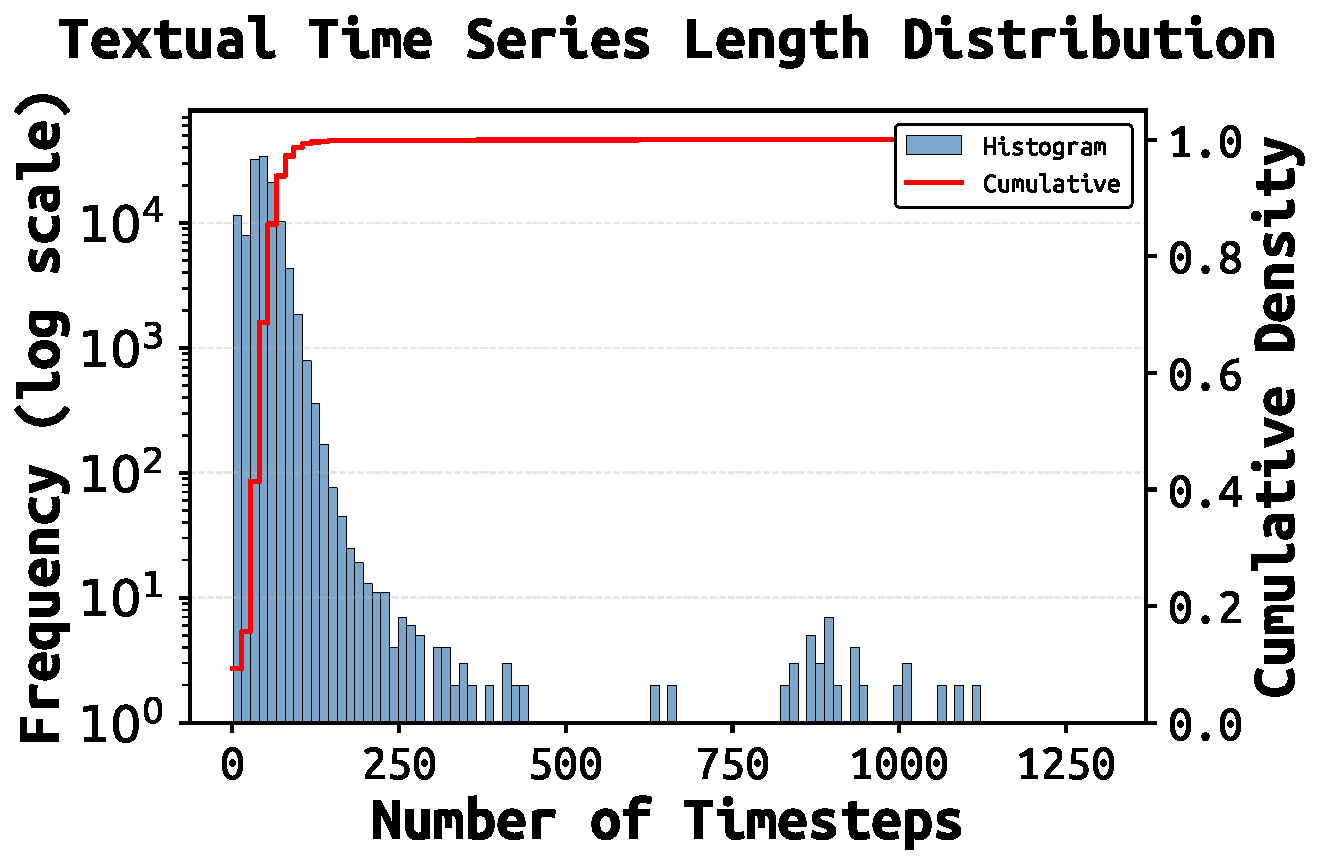
\includegraphics[width=\linewidth]{Plots_tables/tts_length_distribution.pdf}
%         \caption*{(a) Distribution of time series lengths (in timesteps) across the dataset.}
%     \end{minipage}\hfill
%     \begin{minipage}{0.48\textwidth}
%         \centering
%         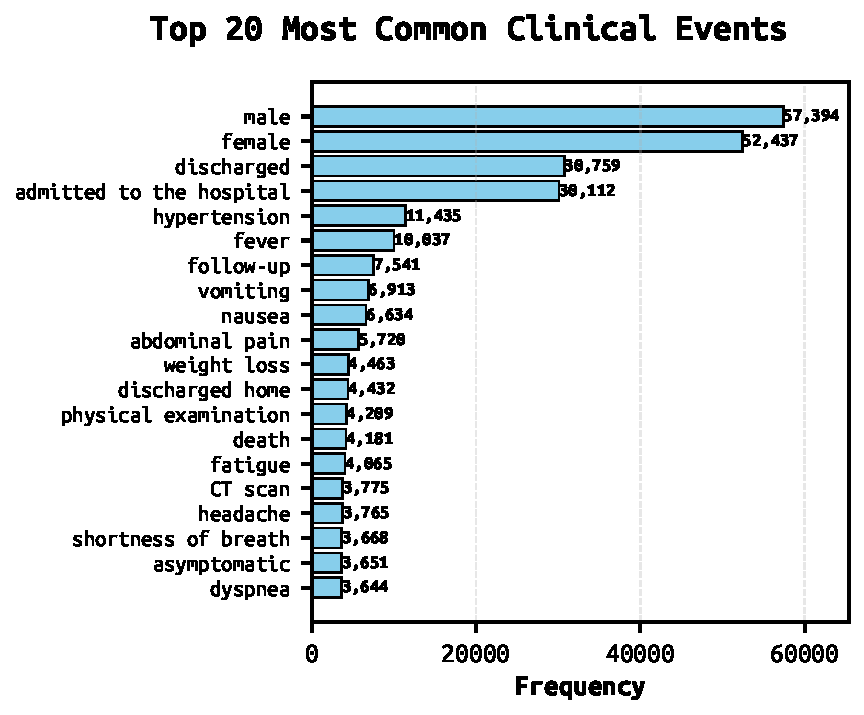
\includegraphics[width=\linewidth]{Plots_tables/top_20_common_events.pdf}
%         \caption*{(b) Most frequently occurring events across all case reports.}
%     \end{minipage}
%     \caption{Overview of textual time series characteristics in the dataset.}
%     \label{fig:tts_stats}
% \end{figure}

%%%%%%%%%%%%%%%%%%%%%%%%%%%
%%%%%%%%%%%%%%%%%%%%%%%%%%%